\documentclass[a4paper,11pt]{article}
\usepackage{amsmath,amsthm,amsfonts,amssymb,amscd,amstext,vmargin,graphics,graphicx,tabularx,multicol} 
\usepackage[francais]{babel}
\usepackage[utf8]{inputenc}  
\usepackage[T1]{fontenc} 
\usepackage{pstricks-add,tikz,tkz-tab,variations}
\usepackage[autolanguage,np]{numprint} 

\setmarginsrb{1.5cm}{0.5cm}{1cm}{0.5cm}{0cm}{0cm}{0cm}{0cm} %Gauche, haut, droite, haut
\newcounter{numexo}
\newcommand{\exo}[1]{\stepcounter{numexo}\noindent{\bf \underline{Exercice~\thenumexo}}}
\reversemarginpar


\newcounter{enumtabi}
\newcounter{enumtaba}
\newcommand{\q}{\stepcounter{enumtabi} \theenumtabi.  }
\newcommand{\qa}{\stepcounter{enumtaba} (\alph{enumtaba}) }
\newcommand{\initq}{\setcounter{enumtabi}{0}}
\newcommand{\initqa}{\setcounter{enumtaba}{0}}

\newcommand{\be}{\begin{enumerate}}
\newcommand{\ee}{\end{enumerate}}
\newcommand{\bi}{\begin{itemize}}
\newcommand{\ei}{\end{itemize}}
\newcommand{\bp}{\begin{pspicture*}}
\newcommand{\ep}{\end{pspicture*}}
\newcommand{\bt}{\begin{tabular}}
\newcommand{\et}{\end{tabular}}
\renewcommand{\tabularxcolumn}[1]{>{\centering}m{#1}} %(colonne m{} centrée, au lieu de p par défault) 
\newcommand{\tnl}{\tabularnewline}

\newcommand{\bmul}[1]{\begin{multicols}{#1}}
\newcommand{\emul}{\end{multicols}}

\newcommand{\trait}{\noindent \rule{\linewidth}{0.2mm}}
\newcommand{\hs}[1]{\hspace{#1}}
\newcommand{\vs}[1]{\vspace{#1}}

\newcommand{\N}{\mathbb{N}}
\newcommand{\Z}{\mathbb{Z}}
\newcommand{\R}{\mathbb{R}}
\newcommand{\C}{\mathbb{C}}
\newcommand{\Dcal}{\mathcal{D}}
\newcommand{\Ccal}{\mathcal{C}}
\newcommand{\mc}{\mathcal}

\newcommand{\vect}[1]{\overrightarrow{#1}}
\newcommand{\ds}{\displaystyle}
\newcommand{\eq}{\quad \Leftrightarrow \quad}
\newcommand{\vecti}{\vec{\imath}}
\newcommand{\vectj}{\vec{\jmath}}
\newcommand{\Oij}{(O;\vec{\imath}, \vec{\jmath})}
\newcommand{\OIJ}{(O;I,J)}




\newcommand{\reponse}[1][1]{%
\multido{}{#1}{\makebox[\linewidth]{\rule[0pt]{0pt}{20pt}\dotfill}
}}

\newcommand{\titre}[5] 
% #1: titre #2: haut gauche #3: bas gauche #4: haut droite #5: bas droite
{
\noindent #2 \hfill #4 \\
#3 \hfill #5

\vspace{-1.6cm}

\begin{center}\rule{6cm}{0.5mm}\end{center}
\vspace{0.2cm}
\begin{center}{\large{\textbf{#1}}}\end{center}
\begin{center}\rule{6cm}{0.5mm}\end{center}
}



\begin{document}
\pagestyle{empty}
\titre{Chapitre 12 : Proportionnalité}{}{}{}{}

\vspace*{1cm}

\begin{center}
{\Large \textbf{Niveau 1 :}}
\end{center}

\vspace*{1cm}

$\rightarrow$ \textbf{La proportionnalité}\\

\vspace*{0.5cm}




\exo \\ Pour chaque situation, cliquer sur la bonne réponse.\\

\renewcommand{\arraystretch}{1.8}

\begin{tabular}{|p{5.5cm}|p{3.5cm}|p{3.5cm}|p{3.5cm}|}
\hline 
   Jean achète trois fois plus de bonbons que Mélanie. Il paiera ... & trois fois moins cher que Mélanie & 3 euros de plus que Mélanie  & 3 fois plus cher que Mélanie \\ 
\hline 
 Aurélie achète deux stylos de plus que Céline. Elle paiera ... & deux fois plus cher que Céline & on ne peut pas savoir & 2 euros de plus que Céline \\ 
\hline 
\end{tabular} 

\vspace*{0.5cm}

\exo \\ 6 stylos coûtent 9 euros.\\

\initqa \qa Combien coûtent 18 stylos ? .......................... \\ 

\qa Combien coûtent 3 stylos ? .......................... \\ 

\qa Combien coûtent 21 stylos ? .......................... \\ 



\exo \\ Voici la recette d'un gâteau pour 6 personnes.\\

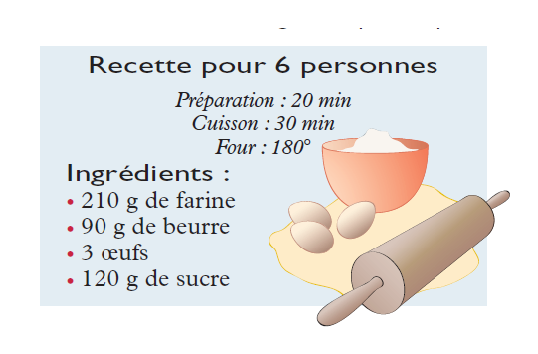
\includegraphics[scale=1]{prop5.eps} \\

Pour faire un gâteau pour 12 personnes, faut-il régler la température du four sur 360\degre ?\\
. . . . . . . . . . . . . \\

\vspace*{1cm}

$\rightarrow$ \textbf{Les pourcentages}\\

\vspace*{0.5cm}


\exo \\ Voici ce que l'on peut lire sur un pot de confiture d'abricot : " Contient 50 \% de fruits."\\
Compléter les phrases suivantes : \\

\initqa \qa Dans un pot de 100 g, il y a  . . . . g d'abricots.\\

 \qa Dans un pot de 200 g, il y a  . . . . g d'abricots.\\


 \qa Dans un pot de 500 g, il y a  . . . . g d'abricots.\\



\exo \\ Blogs et pourcentages\\

" Fin 2005, un Français sur dix avait déjà créé un blog et environ un sur quatre en avait déjà visité un blog "\\

Compléter cette phrase avec des pourcentages.\\

" Fin 2005 ..........................\% des français avaient déjà créé un blog et .................................... \% en avaient visité un. »\\




 \exo \\ Calculer comme sur l'exemple, les pourcentages ci-dessous.\\
 
\textbf{ Exemple :}  10 \% de 62 = $\dfrac{10}{100} \times 62 = \dfrac{62 \times 10 }{100} = \dfrac{620}{100} = 6,2$\\

\initqa \qa 10 \% de 50 = . . . .\\

\qa 15 \% de 200 = . . . .\\

\qa 82 \% de 100 = . . . .\\

\qa 25 \% de 300 = . . . .\\











\vspace*{0.5cm}

\begin{center}
{\Large \textbf{Niveau 2 :}}
\end{center}

\vspace*{1cm}

$\rightarrow$ \textbf{La proportionnalité}\\

\vspace*{0.5cm}


\exo \\ Pour chaque situation, cliquer sur la bonne réponse.\\

\renewcommand{\arraystretch}{1.8}

\begin{tabular}{|p{7.5cm}|p{2.5cm}|p{3.5cm}|p{3.5cm}|}
\hline 
  Mon arrosoir contient 10 L et celui de mon petit frère Yann contient 5 L. J'ai transporté 6 arrosoirs pleins jusqu'au jardin. Pour en transporter autant que moi, Yann devra remplir complètement ...   & 9 arrosoirs & 12 arrosoirs  & 3 arrosoirs \\ 
\hline 
 Maman avait prévu le goûter pour nous trois mais mes cousins sont arrivés et nous étions alors six pour le partager. La part de chacun : ... & n'a pas changé. & est deux fois plus grande. & est deux fois plus petite. \\ 
\hline 
\end{tabular} 


\exo \\ Compléter le tableau de proportionnalité suivant: \\ 

\includegraphics[scale=1]{prop2.eps} \\





\exo \\ Cliquer sur la bonne réponse.\\

\begin{tabular}{|p{7cm}|p{3.5cm}|p{3.5cm}|}
\hline 
\textbf{Situation} & \multicolumn{2}{c|}{\textbf{La situation est-elle proportionnelle ?}} \\ 
\hline 
Jane a 10 ans et son père 36 an. Quand Jane aura 30 ans, quel âge aura son père ? & oui & non \\ 
\hline 
Une moto consomme en moyenne 4 litres d'essence pour 100 km. Quelle sera sa consommation pour 350 km? & oui & non \\ 
\hline 
Maxime pèse 32 kg à 10 ans. Combien pèsera-t-il à 20 ans ? & oui & non \\ 
\hline 
\end{tabular} 



\vspace*{1cm}

$\rightarrow$ \textbf{Les pourcentages}\\

\vspace*{0.5cm}



\exo \\ Voici ce que l'on peut lire sur un pot de confiture d'abricot : " Contient 35 \% de fruits."\\
Compléter les phrases suivantes : \\

\initqa \qa Dans un pot de 100 g, il y a  . . . . g d'abricots.\\

 \qa Dans un pot de 200 g, il y a  . . . . g d'abricots.\\


 \qa Dans un pot de 500 g, il y a  . . . . g d'abricots.\\




 \exo \\ Calculer comme sur l'exemple, les pourcentages ci-dessous.\\
 
\textbf{ Exemple :}  10 \% de 62 = $\dfrac{10}{100} \times 62 = \dfrac{62 \times 10 }{100} = \dfrac{620}{100} = 6,2$\\

\initqa \qa 75 \% de 200 = . . . .\\

\qa 80 \% de 60 = . . . .\\

\qa 2,5 \% de 400 = . . . .\\

\qa 19 \% de 50 = . . . .\\


\exo \\ Julie obtient une réduction de 15 \% sur un vélo valant 158 euros. Quel est le montant de la réduction obtenue par Julie ?\\



Calculs :\\
\reponse[2]\\


Réponse :\\
\reponse[1]\\




\exo \\ Durant un match de basket, Yann a réussi 80 \% de ses tirs. Il a effectué 50 tirs. Combien de paniers a-t-il marqué ?\\

Calculs :\\
\reponse[2]\\


Réponse :\\
\reponse[1]\\







\begin{center}
{\Large \textbf{Niveau 3 :}}
\end{center}

\vspace*{1cm}

$\rightarrow$ \textbf{La proportionnalité}\\

\vspace*{0.5cm}





\exo \\ Pour chaque situation, cliquer sur la bonne réponse.\\

\renewcommand{\arraystretch}{1.8}

\begin{tabular}{|p{7.5cm}|p{2.5cm}|p{3.5cm}|p{3.5cm}|}
\hline 
  Maman avait prévu le goûter pour nous trois mais mes cousins sont arrivés et nous étions alors six pour le partager. La part de chacun : ... & n'a pas changé. & est deux fois plus grande. & est deux fois plus petite. \\
\hline 
    Dans une librairie, Maxime a acheté 8 BD pour 22 euros et Anne a acheté 6 BD pour 18 euros. & On est sûr que le prix en euros de 14 BD est 22 + 18 euros. & On est sûr que le prix en euros de 2 BD est 22 - 18 euros & On ne peut rien affirmer sur le prix de 2 BD prises au hasard. \\
\hline 
\end{tabular} 




\exo \\ Compléter le tableau de proportionnalité suivant: \\ 

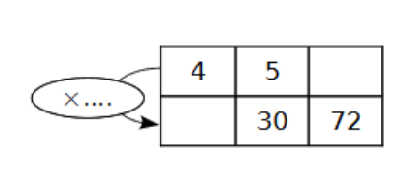
\includegraphics[scale=1]{prop3.eps} \\


\exo \\ Le tableau de proportionnalité suivant indique la consommation moyenne d'un véhicule en fonction de la distance parcourue. Compléter le tableau ci-dessous.\\


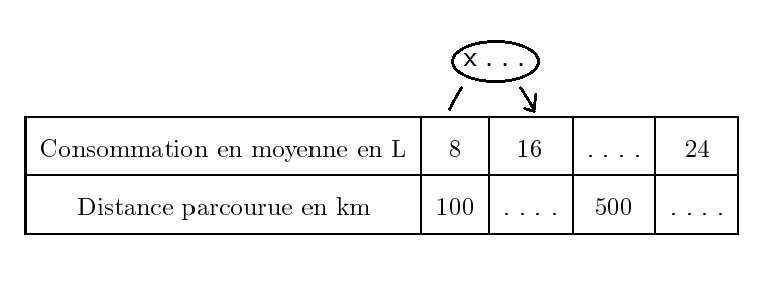
\includegraphics[scale=1]{prop4.eps} \\




\exo \\ Pour chaque tableau ci-dessous, indiquer si les grandeurs considérées sont proportionnelles.\\

\begin{tabular}{|c|c|c|c|}
\hline 
Nombre de cahiers & 2 & 3 & 7 \\ 
\hline 
Prix en euros & 6 & 9 & 21 \\ 
\hline 
\end{tabular}\hspace*{4cm} \begin{tabular}{|c|c|c|c|}
\hline 
Nombre d'avocats & 2 & 3 & 5 \\ 
\hline 
Prix en euros & 4 & 6 & 8 \\ 
\hline 
\end{tabular} 


oui / non \hspace*{8cm} oui / non\\




\vspace*{1cm}

$\rightarrow$ \textbf{Les pourcentages}\\

\vspace*{0.5cm}




\exo \\ Les jeunes de 11 à 14 ans passent en moyenne 12,5 \% d'une journée (24h) devant un écran.\\
70 \% de ce temps est passé devant la télévision et le reste du temps devant un ordinateur.\\

Combien d'heures les jeunes de 11 à 14 ans passent-ils en moyenne chaque jour devant  un écran ?\\


Calculs :\\
\reponse[2]\\


Réponse :\\
\reponse[1]\\



\exo \\ Les jeunes de 11 à 14 ans passent en moyenne 12,5 \% d'une journée (24h) devant un écran.\\
70 \% de ce temps est passé devant la télévision et le reste du temps devant un ordinateur.\\

Combien d'heures les jeunes de 11 à 14 ans passent-ils en moyenne chaque jour devant  la télévision ?\\


Calculs :\\
\reponse[2]\\


Réponse :\\
\reponse[1]\\




\exo \\ Julie obtient une réduction de 15 \% sur un vélo valant 158 euros. Quel est le nouveau prix du vélo après la réduction ?\\



Calculs :\\
\reponse[2]\\


Réponse :\\
\reponse[1]\\


\exo \\ L'effectif d'un collège de 800 élèves va augmenter de 5 \% l'année prochaine.\\
Calculer le nombre d'élèves qu'il y aura à la rentrée prochaine.\\



Calculs :\\
\reponse[2]\\


Réponse :\\
\reponse[1]\\







\begin{center}
{\Large \textbf{Niveau 4:}}
\end{center}

\vspace*{1cm}

$\rightarrow$ \textbf{La proportionnalité}\\

\vspace*{0.5cm}

\exo \\ Un morceau de ficelle de 4 m coûte 3,60 euros. \\
Compléter le tableau de proportionnalité suivant.\\

\begin{tabular}{|c|c|c|c|c|c|}
\hline 
Longeur en m & 4 & 8 & 12 & 3 & 15 \\ 
\hline 
Prix en euros & 3,60 & . . . . & . . . . & . . . . & . . . . \\ 
\hline 
\end{tabular} 



\exo \\ Le son du tonnerre parcourt 900 m en 3 s.\\
On souhaite savoir quelle distance parcourt le son du tonnerre en 5 secondes, pour cela il faut compléter le tableau de proportionnalité ci-dessous.\\

\begin{tabular}{|c|c|c|}
\hline 
Durée en s & 3 & 5 \\ 
\hline 
Distance en m & 900 & . . . .  \\ 
\hline 
\end{tabular} 




\exo \\ Le son du tonnerre parcourt 900 m en 3 s.\\
On souhaite savoir quel temps met le son du tonnerre pour parcourir 450 m, pour cela il faut compléter le tableau de proportionnalité ci-dessous.\\

\begin{tabular}{|c|c|c|}
\hline 
Durée en s & 3 & . . . . . \\ 
\hline 
Distance en m & 900 & 450 \\ 
\hline 
\end{tabular} 




\exo \\ Pour chaque tableau ci-dessous, indiquer si les grandeurs considérées sont proportionnelles.\\

\begin{tabular}{|p{5cm}|c|c|c|c|}
\hline 
Quantité de pommes de terre (en kg) & 1 & 3 & 5 & 10 \\ 
\hline 
Prix (en euros) & 0,50 & 1,50 & 2,40 & 5 \\ 
\hline 
\end{tabular}\hspace*{1cm} \begin{tabular}{|c|c|c|c|}
\hline 
Volume de béton ($m^{3}$) & 1 & 4 & 6 \\ 
\hline 
Masse de ciment (kg) & 355 & 1 420 & 2 130\\ 
\hline 
\end{tabular} 

\vspace*{0.5cm}

oui / non \hspace*{10cm} oui / non\\



\vspace*{1cm}

$\rightarrow$ \textbf{Les pourcentages}\\

\vspace*{0.5cm}



\exo \\ Les jeunes de 11 à 14 ans passent en moyenne 12,5 \% d'une journée (24h) devant un écran.\\
70 \% de ce temps est passé devant la télévision et le reste du temps devant un ordinateur.\\

Combien d'heures les jeunes de 11 à 14 ans passent-ils en moyenne chaque jour devant  un ordinateur ?\\


Calculs :\\
\reponse[2]\\


Réponse :\\
\reponse[1]\\





\exo \\ Dans une commune, 588 personnes ont une licence sportive. Le tableau concerne cinq des disciplines les plus pratiquées, et le pourcentage de femmes est celui parmi les adhérents de la discipline pratiquée.\\
Compléter le tableau ci-dessous.\\


\begin{tabular}{|c|c|c|c|c|}
\hline 
Fédération & \% & Nombre d'adhérents & \% de femmes & Nombre de femmes \\ 
\hline 
Football & 29,93 & . . . . & 4,55 & . . . . \\ 
\hline 
Tennis & 14,29 & . . . . & 33,33 & . . . . \\ 
\hline 
Judo  & 6,8 & . . . . & 30 & . . . . \\ 
\hline 
Equitation & 6,8 & . . . . & 80 & . . . . \\ 
\hline 
Basketball & 5,44 & . . . . & 37,5 & . . . . \\ 
\hline 
\end{tabular} 


\exo \\ Dans le collège Camus, on a posé la question suivante aux élèves : " Quel est l'équipement informatique disponible dans votre maison ?" \\
On a obtenu ces résultats (arrondis au centième).\\

\begin{tabular}{|c|c|}
\hline 
Un ordinateur + internet avec accès libre  & 62,67 \% \\ 
\hline 
Un ordinateur + internet avec accès limité  & 14,75 \% \\  
\hline 
Un ordinateur + internet avec les parents  & 11,06 \% \\   
\hline 
Un ordinateur sans  internet  & 6,91 \% \\ 
\hline 
Pas d'ordinateur & . . . . \\ 
\hline 
TOTAL & . . . . \\ 
\hline 
\end{tabular} 

Compléter alors les cases manquantes.\\







\begin{center}
{\Large \textbf{Niveau 5 :}}
\end{center}

\vspace*{1cm}

$\rightarrow$ \textbf{La proportionnalité}\\

\vspace*{0.5cm}






\exo \\ Le son du tonnerre parcourt 900 m en 3 s.\\
On souhaite savoir quel temps met le son du tonnerre pour parcourir 3,5 km, pour cela il faut compléter le tableau de proportionnalité ci-dessous.\\

\begin{tabular}{|c|c|c|}
\hline 
Durée en s & 3 & . . . . . \\ 
\hline 
Distance en m & 900 & . . . . . \\ 
\hline 
\end{tabular} 




\exo \\ Compléter le tableau de proportionnalité suivant qui donne le prix de l'essence  en fonction de la quantité achetée.\\


\begin{tabular}{|c|c|c|c|c|c|}
\hline 
Nombre de litres d'essence achetées & 1 & 12 & . . . .  & . . . . . & 75 \\ 
\hline 
Prix en euros & 1,2 & . . . . & 30 & 360 & . . . . \\ 
\hline 
\end{tabular} 




\exo \\ Voici la recette d'un gâteau pour 6 personnes.\\

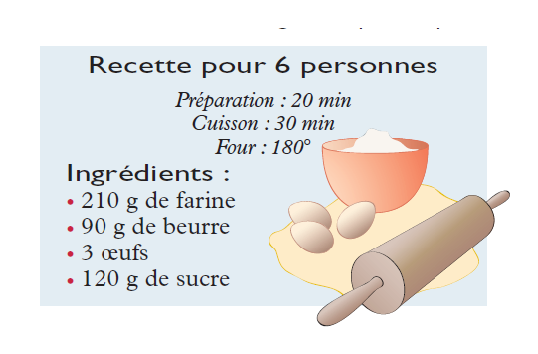
\includegraphics[scale=1]{prop5.eps} \\

Quelle est la quantité de chaque ingrédient nécessaire à l'élaboration d'un gâteau pour 10 personnes ?\\


farine : . . . . .\\
beurre : . . . . . \\
oeufs : . . . . .\\
sucre : . . . . .\\


\exo \\ Pour chaque tableau ci-dessous, indiquer si les grandeurs considérées sont proportionnelles.\\

\begin{tabular}{|c|c|c|c|c|}
\hline 
Quantité de fraises (en kg) & 1 & 3 & 5 & 10 \\ 
\hline 
Prix (en euros) & 0,40 & 1,20 & 2 & 4\\ 
\hline 
\end{tabular}\hspace*{1.5cm} \begin{tabular}{|c|c|c|}
\hline 
 1,5 & 4,5 & 6 \\ 
\hline 
2,5 & 7,5 & 10,5\\ 
\hline 
\end{tabular} 

\vspace*{0.5cm}

oui / non \hspace*{8cm} oui / non\\



\vspace*{1cm}

$\rightarrow$ \textbf{Les pourcentages}\\

\vspace*{0.5cm}



\exo \\ Pendant un vide grenier, Zoé a réussi à vendre 54 de ses 72 BD. Quel pourcentage de ses BD a-t-elle vendues ?\\
Pour répondre à cette question, compléter le tableau de proportionnalité ci-dessous.\\

\begin{tabular}{|c|c|c|}
\hline 
Nombre de BD & 72 & 54 \\ 
\hline 
Pourcentage & 100 & . . . . \\ 
\hline 
\end{tabular} 



Calculs :\\
\reponse[2]\\


Réponse :\\
\reponse[1]\\


\exo \\ Dans une classe de 24 élèves, 9 sont demi-pensionnaires. Calculer le pourcentage d'élèves demi-pensionnaires.\\



Calculs :\\
\reponse[2]\\


Réponse :\\
\reponse[1]\\



\exo \\ Dans le collège Camus, on a posé la question suivante à 217 élèves : " Quel est l'équipement informatique disponible dans votre maison ?" \\
On a obtenu ces résultats (arrondis au centième).\\

\begin{tabular}{|c|c|}
\hline 
Un ordinateur + internet avec accès libre  & 62,67 \% \\ 
\hline 
Un ordinateur + internet avec accès limité  & 14,75 \% \\  
\hline 
Un ordinateur + internet avec les parents  & 11,06 \% \\   
\hline 
Un ordinateur sans  internet  & 6,91 \% \\ 
\hline 
Pas d'ordinateur & 4,61 \% \\ 
\hline 
TOTAL & 100 \% \\ 
\hline 
\end{tabular} \\


On souhaite savoir combien d'élèves sont concernés pour chacune des réponses, compléter alors le tableau ci-dessous.\\


\begin{tabular}{|c|c|}
\hline 
Réponse  & Nombre d'élèves \\ 
\hline 
Un ordinateur + internet avec accès libre  & . . . . . \\ 
\hline 
Un ordinateur + internet avec accès limité  & . . . . . \\ 
\hline 
Un ordinateur + internet avec les parents  & . . . . . \\ 
\hline 
Un ordinateur sans  internet  & . . . . . \\ 
\hline 
Pas d'ordinateur & . . . . . \\ 
\hline 
TOTAL & . . . . . \\ 
\hline 
\end{tabular} 


\end{document}
